% experimentacion
\vspace{0.5em}
Para revisar empíricamente la cota lineal del algoritmo estipulado, primero tomamos los tiempos de ejecución de muestras aleatorias de tamaños de potencias de 2, desde la decimosexta hasta la vigésimosexta.

Luego graficamos el tiempo de ejecución de en función de estos tamaños de entrada, aplicando el logaritmo en ambas entradas para mejorar la visibilidad, dada la naturaleza exponencial de las muestras. Tras aplicar regresión lineal, el gráfico quedó de la siguiente forma:

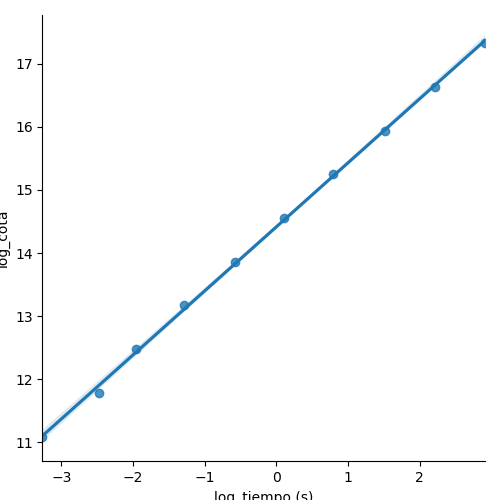
\includegraphics{files/src/.media/Grafico_aleatorios.png}

La relación lineal es bastante clara, pero calculamos también el coeficiente de Pearson para asegurarnos. Queda 0.9996692305026845, muy cercano a 1.

\vspace{0.5em}
% instancias
\subsection{Instancias de interés}

Lo único que parece alterar el flujo del código en función de la entrada es si cada tupla ordenada empieza después (o al mismo tiempo) que cuando termina la última tarea de P. En ese caso se ejecutan dos lineas más, aunque tienen tiempo de ejecución constante y no parecen ser demasiado significativas.

Para probar la diferencia de tiempos entre instancias, hacemos el mismo test de la sección anterior, primero con una instancia comprimida en la que la intersección entre todos los intervalos es no vacía (sólo se entra al if en la primera ejecución del ciclo) y luego una instancia de entradas separadas donde la i-ésima entrada tiene la forma (i,i+1), por lo que siempre se entra al if. El gráfico queda de la siguiente forma:

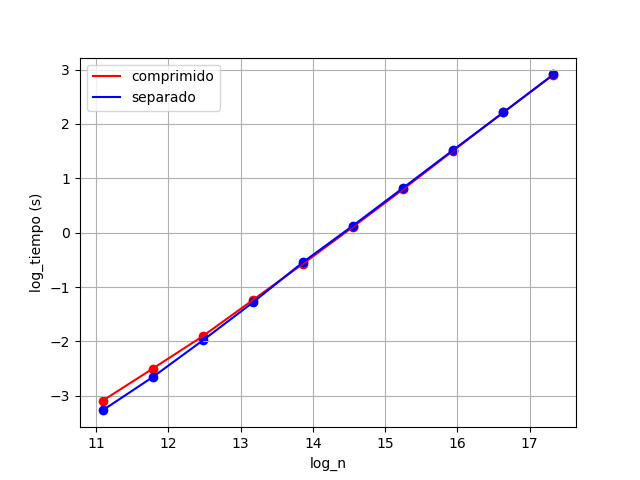
\includegraphics{files/src/.media/Grafico_comprimido_vs_separado.png}

Si bien es verdad que en las entradas más grandes el sample de entradas separdas parece haber tomado un poco más de tiempo, no resulta una diferencia significativa.